\documentclass{amsart}
\usepackage{fullpage}

\usepackage[T1]{fontenc}
\usepackage[utf8]{inputenc} 
\usepackage{lmodern}
\usepackage[slovene]{babel}
\usepackage{amsmath,amssymb,amsfonts}
\usepackage{bbm}
\usepackage{graphicx}
\graphicspath{{./images/}}

\linespread{1.2}

\newcommand{\N}{\mathbb{N}}
\newcommand{\Z}{\mathbb{Z}}
\newcommand{\Q}{\mathbb{Q}}
\newcommand{\R}{\mathbb{R}}
\newcommand{\C}{\mathbb{C}}

% ukazi za matematicna okolja
\theoremstyle{definition} % tekst napisan pokoncno
\newtheorem{definicija}{Definicija}[section]
\newtheorem{primer}[definicija]{Primer}
\newtheorem{opomba}[definicija]{Opomba}

\renewcommand\endprimer{\hfill$\diamondsuit$}


\theoremstyle{plain} % tekst napisan posevno
\newtheorem{lema}[definicija]{Lema}
\newtheorem{izrek}[definicija]{Izrek}
\newtheorem{trditev}[definicija]{Trditev}
\newtheorem{posledica}[definicija]{Posledica}

\title{Kontekstno-neodvisne gramatike za kodiranje in stiskanje podatkov}
\author{Janez Podlogar}
\date{\today}

\begin{document}

\begin{abstract}
    V naslovu se pojavijo trije pomembni pojmi. Kodiranje podatkov, stiskanje
    podatkov in kontekstno-neodvisne gramatike.
\end{abstract}

\maketitle

\section{Kodiranje podatkov}

Zapis informacije v neki obliki ni primeren za vsakršno rabo. Besedilo, zapisano z 
pismenkami, je neberljivo za slepe osebe, saj je komunikacijski kanal v tem primeru
vid. Pisanega besedila v pravotni obliki ni moč poslati z telegrafom. V tem primeru
je komunikacijski kanal žica in pismenke se po njej ne morejo sprehoditi. V obeh 
primerih je informacija, ki bi jo radi prenesli v neprimerni obliki. V prvem 
primeru je potrebno besedilo zapisati z Braillovo pisavo. V drugem primeru pa je 
potrebno besedil pretvoriti v električni signal. Spreminjanje zapisa sporočila
pravimo \textit{kodiranje}, sistemu pravil, po katerem se kodiranje opravi,
pa \textit{kod}. 

\begin{primer}
    \textit{Morsejeva abeceda} je kodiranje črk, števil in ločil s pomočjo zaporedja kratkih
    in dolgih signalov:

    \begin{itemize}
        \item Dolžina kratkega signala je ena enota.
        \item Dolgi signal je trikrat daljši od kratkega signala.
        \item Razmiki med signali znotraj znaka so dolžine kratkega signala.
        \item Presledki med znaki so dolgi tri kratke signale oz. en dolgi signal.
        \item Presledki med besedami so dolgi sedem kratkih signalov.
    \end{itemize}

    \begin{figure}[h]
        \centering
        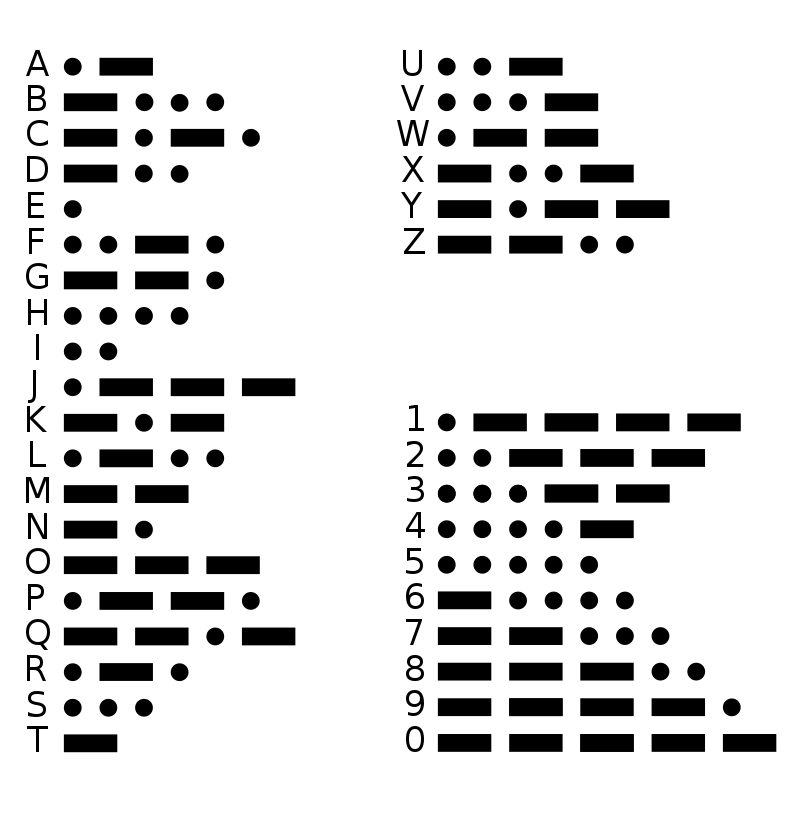
\includegraphics[width=4.5cm]{International_Morse_Code.svg.png}
        \caption{Mednarodna Morsejeva abeceda}
    \end{figure}

    Kodiranje črk je takšno, da imajo črke z višjo frekvenco (v angleškem jeziku)
    krajši zapis. 
    
    Prvotni namen Morsejeve abecede je komunikacija preko telegrama, saj komunikacijski
    kanal dovoljuje le električne signale in tišino med njimi. 
 

\end{primer}

\section{Kompresija podatkov}

\section{Kontekstno-neodvisne gramatike}

\end{document} 